%
% Thesis Style 用サンプル TeX
%
% 注意:目次等を作成するために何度か platex にかけること
%
% 両面印刷する時は twoside にする
%
% 12pt にするのは最終手段
%
\documentclass[11pt,oneside]{jbook}
\usepackage{csg-thesis}
\usepackage{graphicx,url}
\usepackage{xcolor}


%%%% macros to add comments
\newif\ifdraftComments
\draftCommentsfalse
\def\mkDraftFn#1#2{%
  \expandafter\def\csname #1\endcsname##1{\ifdraftComments\textcolor{#2}{[#1: ##1]}\marginpar[$\longrightarrow$]{$\longleftarrow$}\fi}%
}
\mkDraftFn{MY}{blue}
\mkDraftFn{YT}{red}
\mkDraftFn{YC}{red}
\mkDraftFn{HM}{red}

\draftCommentstrue



\begin{document}

% 題目
% 適当に\\で区切って見やすくする
\title{%
かっこいい\\
タイトル
}

% 学位(学部と大学院で変更)
\degree{学士}
%\degree{修士}

% 名前
\author{著者名}

% 提出日
\date{令和y年m月d日}

% 卒業年度
\schoolyear{令和y年}

% 所属(学部と大学院で変更)
% \department{東京工業大学 理学部 情報科学科}
\department{%
% 学部
東京科学大学 情報理工学院\\
数理・計算科学系
% 修士
% 東京科学大学 情報理工学院\\
% 数理・計算科学系 数理・計算科学コース
}

% 学籍番号
\stnumber{xx-xxxx-x}

% 指導教員
\supervisor{増原 英彦 教授}
% \supervisor{叢 悠悠 助教}

\maketitle

%%%%%%%%%%%%%%%%%%%%%%%%%%%%%%%%%%%%%%%%%%%%%%%%%%%%%%%%%%%%%%%%%%%%%%

% 概要
\begin{abstract}
本稿は、プログラム分散化のためのアスペクト指向言語(AOP)であるAddistant%
を拡張した、Addistant 2を提案する。Addistantは、利用者が分散に関する記述
を独自のアスペクト指向言語で指定することにより、単一のJava仮想機械(JVM)
上で実行することを目的として開発した既存プログラムを、利用者が望む形で機
能分散化を導入する。この分散化はロード時に、バイトコードレベルで行われる。
Addistant 2は、分散アスペクトの記述力が十分ではなかったAddistantを、分散
アスペクトのJoin pointの種類を増加することにより、大幅に分散アスペクトの
記述力を強化した。また、本稿はAddistant 2の典型的な利用方法の例も示す。

\end{abstract}

% 謝辞
\begin{acknowledgments}
% ちょっとくだけすぎかも
本稿は以下の方々なくして、存在しえなかったでしょう。
Addistant の開発、Addistant 2 の提案および本稿の編集になにかと心を砕いて
いただいた千葉滋講師、東京大学の光来健一氏、筑波大学の立堀道昭氏、横田
大輔氏そして研究室のみなさん。
心より感謝しています。

(具体的に何をしてもらったか書く)

\end{acknowledgments}

%%%%%%%%%%%%%%%%%%%%%%%%%%%%%%%%%%%%%%%%%%%%%%%%%%%%%%%%%%%%%%%%%%%%%%

\tableofcontents       %% 目次

%
% 目次等にはローマ数字を使い、本文開始ページを 1 ページ目にできる
% この方が見た目がきれいであるが、全体のページ数は減って見える
% ここでローマ数字に変えた場合は chapter 1 でアラビア数字に戻すこと
%
\pagenumbering{roman}  %% ページ番号をローマ数字にする

\listoffigures         %% 図目次(図がない場合は不要)
\listoftables          %% 表目次(表がない場合は不要)

%%%%%%%%%%%%%%%%%%%%%%%%%%%%%%%%%%%%%%%%%%%%%%%%%%%%%%%%%%%%%%%%%%%%%%

\cleardoublepage
\pagenumbering{arabic}  %% ページ番号をローマ数字にする
%
% 本文
%
% 各章を各ファイルに書く
%
\chapter{はじめに}
%\pagenumbering{arabic}  %% ページ番号をアラビア数字に変更

今日、分散ソフトウェア、つまり複数の計算機上で動作するソフトウェアの必要
性が高まる一方、その開発にかかるコストが問題になっている。これは、分散プ
ログラムを作成する場合にネットワークなどの分散環境特有の問題に対処しなけ
ればならないためである。それらの処理の記述を含んだ分散プログラムは煩雑に
なり、非分散プログラムの作成に比べて、分散プログラムの作成や維持にかかる
人的コストは飛躍的に大きくなりがちである。

分散プログラミングが煩雑であることの要因として、プログラムの分散に無関係
な記述の中に分散に関わる処理が拡散して入り交じっている(crosscutting
concerns)ことがあげられる。このようなプログラムは可読性が低く、変更も大
変である。分散に無関係な記述が分かりにくくなる上、分散に関わる処理を変更
するためにはプログラムのあちこちを修正しなければならなくなる。

我々は分散プログラミングをアスペクト指向言語(AOP)により支援する 
Addistant を開発してきた。ここで、アスペクト指向とは、オブジェクト指向と
の相補性を意識した概念である。オブジェクト指向とは、機能性という点に着目
して全体をオブジェクトと呼ばれるモジュールに分割していく概念である。しか
し、個々のモジュール内には、同様の処理が股がる可能性がある。この個々のモ
ジュールに股がった同様な処理を、オブジェクトとは別の側面から考慮し、それ
をモジュール化する概念を{\bf{アスペクト指向}} といい、そのモジュールを
{\bf{アスペクト}}という。

Addistant は次の特徴をもつ。
%
\begin{itemize}
\item{
Addistant の利用者に、各クラスごとそのオブジェクトを分散環境中のどこに配
置するかを指定させる。Addistant では、分散に関わる処理がプログラム全体に
拡散して入り交じることを避けるため、利用者は、分散に無関係な記述である非
分散プログラムとは別に、分散に関わる記述をまとめて記述する。このまとめて
別に書かれた分散に関わる記述を{\bf{分散アスペクト}}と呼ぶ。
}
\item{
対象プログラムのバイトコードを変換して、分散アスペクトによって指定された
クラスが、遠隔ホストで動作している Java 仮想機械(JVM)上で実行されるよ
うにする。Addistant は変換のために、対象プログラムのソースコードを必要と
しない。変換されたバイトコードは正規の Java バイトコードであり、実行のた
めに特別な JVM を必要としない。バイトコード変換には 
Javassistを用いた。
}
\item{
変換されたバイトコードを Addistant の実行系により遠隔 JVM に自動的に
配布される。
}
\end{itemize}
%
\noindent
Addistant では、遠隔オブジェクト参照を、従来の分散プログラミング・ツール
で使われてきたアイディアを組み合わせて実現した。この実装は、{\bf{プロキ
シ・マスタ方式}}に基づいたもので、Addistant がバイトコード変換により自動
的に行う。

しかしながら、Addistant では、開発が進むにつれ、その利点とともに問題点も
明らかになってきた。その問題点とは、分散アスペクトの記述力が十分ではなかっ
たため、利用者が望む機能分散をうまく実現できない場合があることである。

そこで我々は、Addistant の分散アスペクトの記述力を大幅に高めたAddistant
2を開発中である。本稿では Addistant 2 の典型的な利用方法の例をあげ、分
散アスペクトの新しい記述方法を説明する。

本稿の残りは、次のような構成からなっている。(以下では、Addistant を
Addistant 1 と呼ぶ。)
第 2 章は 分散プログラミング用アスペクト言語の
必要性と Addistant 1 の性能を述べる。
第 3 章では、Addistant 2 の分散アスペクト記述を、
第 4 章では、Addistant 2 のこれまでの実装、
第 5 章では、Addistant 2 を利用したソフトウェアの機能分散例、
第 6 章では、関連研究を、そして
第 7 章でまとめを述べる。

%%%%
\chapter{関連研究}

\section{Javassist}

% 引用の例
Javassist~\cite{Chiba2000,Chiba2001a}は...

Javassistは\cite{Javassist}で配布されている。

\section{Addistant}


%%%%
\chapter{Addistant 2 - 記述力強化版}


%%%%
\chapter{実装}

% 図の例
\begin{figure}[tb]
 \begin{center}
  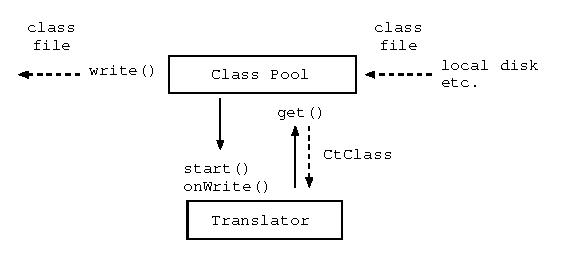
\includegraphics[width=10cm]{javassist.eps}
  \caption{Javassistの処理の流れ}
  \label{fig:javassist}
 \end{center}
\end{figure}

図~\ref{fig:javassist}は...


%%%%
\chapter{実験}

% 表の例
\begin{table}[tb]
 \begin{center}
  \caption{Addistant 2の実行時間(秒)}
  \label{tab:time}
  \begin{tabular}{lr}
   \hline
                   & 時間 \\
   \hline
   X Window System & 15.0 \\
   Addistant 1     &  3.0 \\
   Addistant 2     &  2.0 \\
   \hline
  \end{tabular}
 \end{center}
\end{table}

表~\ref{tab:time}は...



%%%%%%%%%%%%%%%%%%%%%%%%%%%%%%%%%%%%%%%%%%%%%%%%%%%%%%%%%%%%%%%%%%%%%%

%
% 参考文献は直接書いてもいいが、bibtex を使うと便利
%  (1)このサンプルを platex にかける
%  (2)jbibtex thesis
%  (3)さらに platex にかける
%  (4)もう何回か platex にかける
%
\bibliographystyle{csg-thesis}
\bibliography{thesis}  %% thesis.bib というファイルを用意

%%%%%%%%%%%%%%%%%%%%%%%%%%%%%%%%%%%%%%%%%%%%%%%%%%%%%%%%%%%%%%%%%%%%%%

% 付録が必要ならつける
\appendix
\chapter{プログラム例}


\end{document}
